\documentclass[a4paper,10pt]{article}
\usepackage{lamia-pedagogy}

\begin{document}

% =========================================================================
% PAGE 1 : Fiche Enseignant & Démarche Pédagogique
% =========================================================================
\ficheHeader{1 Heure}{\makebox[2.5cm]{\dotfill}}{1\textsuperscript{ère} AM}{2026 / 2027}

\vspace{-3pt}
\competenceBanner{\faComments\ Projet 01 / Séquence 01 — Séance 02 : Production de l'Oral}

\vspace{-2pt}
\modaliteSupportBar{En binômes puis individuel}{Manuel scolaire p. 10 / Support iconique \guillemotleft\ Les 5 étapes du lavage des mains \guillemotright}

\vspace{1pt}

\begin{minipage}[t]{0.485\textwidth}
\begin{tcolorbox}[
  enhanced,
  colback=secondarylight,
  colframe=secondary,
  arc=1.5mm,leftrule=3pt,rightrule=0.5pt,toprule=0.5pt,bottomrule=0.5pt,
  top=3pt,bottom=3pt,left=6pt,right=6pt,
  title={\small\textbf{\faBullseye\ Objectifs d'apprentissage}},
  coltitle=secondary!90!black,attach boxed title to top left={yshift=-2mm,xshift=4mm},
  boxed title style={colback=white,boxrule=0.5pt,colframe=secondary,arc=1mm,top=1pt,bottom=1pt}
]
\vspace{1pt}
{\small
\begin{itemize}[leftmargin=*,noitemsep,topsep=1pt]
  \item[\faCheckCircle] Produire des phrases orales à partir d'un support imagé.
  \item[\faCheckCircle] Nommer les objets et actions de la salle de bain.
  \item[\faCheckCircle] Structurer l'explication chronologiquement.
\end{itemize}
}
\end{tcolorbox}
\end{minipage}%
\hfill
\begin{minipage}[t]{0.485\textwidth}
\begin{tcolorbox}[
  enhanced,
  colback=accentlight!35,
  colframe=accent,
  arc=1.5mm,leftrule=3pt,rightrule=0.5pt,toprule=0.5pt,bottomrule=0.5pt,
  top=3pt,bottom=3pt,left=6pt,right=6pt,
  title={\small\textbf{\faLightbulb\ Connecteurs d'ordre}},
  coltitle=accent!90!black,attach boxed title to top left={yshift=-2mm,xshift=4mm},
  boxed title style={colback=white,boxrule=0.5pt,colframe=accent,arc=1mm,top=1pt,bottom=1pt}
]
\vspace{1pt}
{\small
\textbf{Pour expliquer les étapes :}
\begin{itemize}[leftmargin=*,noitemsep,topsep=1pt]
  \item \textbf{D'abord / Premièrement :} Mouiller les mains.
  \item \textbf{Ensuite / Puis :} Savonner et frotter.
  \item \textbf{Enfin / Pour finir :} Rincer et sécher.
\end{itemize}
}
\end{tcolorbox}
\end{minipage}

\vspace{3pt}

% Boîte à outils lexicale
\begin{tcolorbox}[
  enhanced,
  colback=white,
  colframe=cardborder,
  arc=2mm,boxrule=0.8pt,
  top=4pt,bottom=4pt,left=8pt,right=8pt,
  title={\small\textbf{\textcolor{primary}{\faTools\ Boîte à outils lexicale pour l'expression orale}}},
  coltitle=primary,colbacktitle=primarylight,titlerule=0.5pt,titlerule style=cardborder
]
{\small
\begin{tabularx}{\linewidth}{X X X}
\textbf{\textcolor{secondary}{Noms :}} & \textbf{\textcolor{secondary}{Verbes :}} & \textbf{\textcolor{secondary}{Adjectifs :}} \\
un lavabo, le robinet & mouiller, appliquer & propre, sale \\
le savon liquide & savonner, frotter & hygiénique, sain \\
la serviette, l'eau tiède & rincer abondamment & indispensable \\
les microbes, la saleté & sécher soigneusement & contaminé \\
\end{tabularx}
}
\end{tcolorbox}

\vspace{3pt}

% Déroulement de la séance
\begin{tcolorbox}[
  enhanced,
  colback=neutrallight,
  colframe=cardborder,
  arc=1.5mm,boxrule=0.6pt,
  top=4pt,bottom=4pt,left=7pt,right=7pt,
  title={\small\textbf{\textcolor{primary}{\faChalkboardTeacher\ Déroulement de l'activité en classe}}},
  coltitle=primary,colbacktitle=white,titlerule=0.4pt
]
{\footnotesize
\begin{enumerate}[label=\textbf{\arabic*.},leftmargin=*,noitemsep,topsep=1pt]
  \item \textbf{Phase d'observation (10 min) :} Découverte collective du support iconique. Identification du lieu (la salle de bain) et des gestes.
  \item \textbf{Phase d'analyse (20 min) :} Questionnement dirigé. Comment s'appelle cette partie ? Que fait l'enfant ? Pourquoi utilise-t-il du savon ?
  \item \textbf{Phase de prise de parole (25 min) :} Pratique en binôme. Chaque élève explique à son camarade les 5 étapes dans l'ordre.
\end{enumerate}
}
\end{tcolorbox}

\newpage

% =========================================================================
% PAGE 2 : Fiche Élève (Support Iconique & Pratique Orale)
% =========================================================================
\ficheHeader{1 Heure}{Nom : \makebox[4cm]{\dotfill}}{1\textsuperscript{ère} AM}{Classe : \makebox[1.5cm]{\dotfill}}

\vspace{-3pt}
\competenceBanner{\faImages\ Fiche de Travail : Les 5 Étapes du Lavage des Mains}

\vspace{2pt}

% Support Visuel Intégré
\begin{tcolorbox}[
  enhanced,
  colback=white,
  colframe=secondary,
  arc=2mm,boxrule=0.8pt,
  top=3pt,bottom=3pt,left=4pt,right=4pt,
  title={\small\textbf{\textcolor{secondary!90!black}{\faEye\ Document Support : Les étapes chronologiques du lavage des mains}}},
  colbacktitle=secondarylight,coltitle=secondary!90!black,titlerule=0.5pt
]
\centering
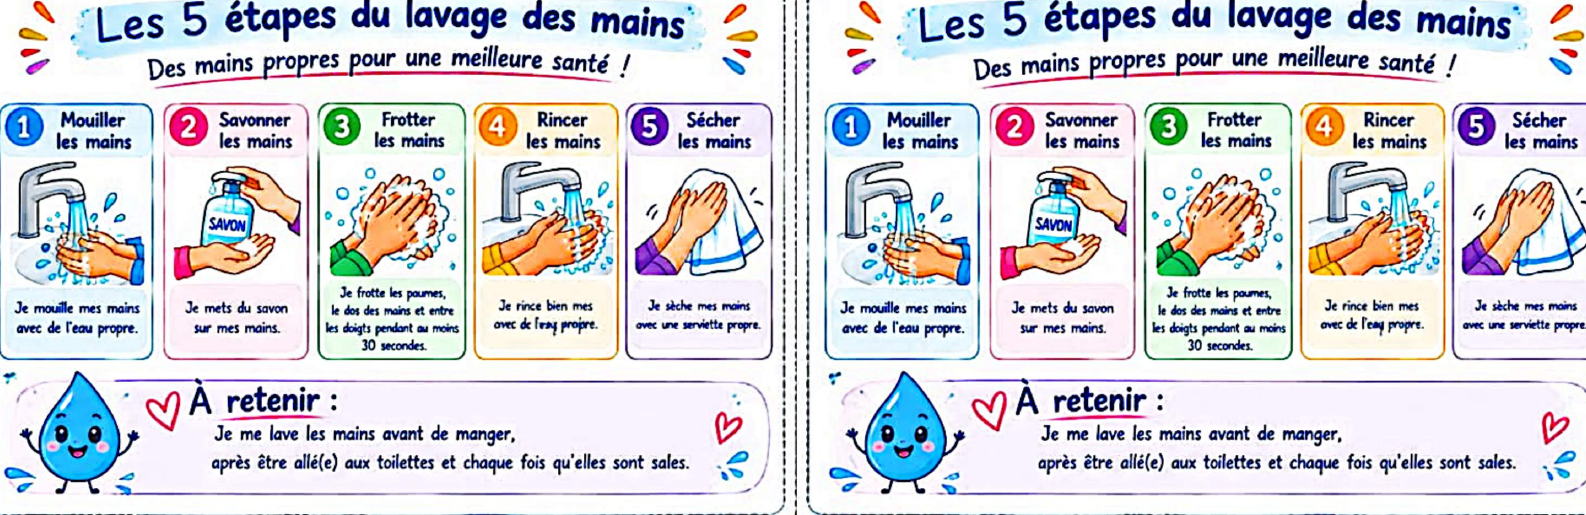
\includegraphics[width=\linewidth,height=5.2cm,keepaspectratio]{assets/images/etapes_lavage_mains.png}
\end{tcolorbox}

\vspace{3pt}

% ACTIVITÉ 1 : Ordre chronologique
\begin{tcolorbox}[
  enhanced,
  colback=white,
  colframe=cardborder,
  arc=2mm,boxrule=0.8pt,
  top=4pt,bottom=4pt,left=8pt,right=8pt,
  title={\small\textbf{\textcolor{primary}{\faListOl\ Activité 01 : Remets les actions dans le bon ordre (de 1 à 5)}} \hfill \badge[primary]{Chronologie}},
  coltitle=primary,colbacktitle=primarylight,titlerule=0.5pt,titlerule style=cardborder
]
{\small
Indique le numéro de l'étape correspondante :
\begin{itemize}[leftmargin=*,noitemsep,topsep=2pt]
  \item[\textbf{[ \phantom{0} ]}] Frotter soigneusement les paumes, le dos des mains et entre les doigts.
  \item[\textbf{[ \phantom{0} ]}] Se sécher les mains avec une serviette propre ou à l'air libre.
  \item[\textbf{[ \phantom{0} ]}] Mouiller les mains avec de l'eau propre.
  \item[\textbf{[ \phantom{0} ]}] Rincer abondamment sous l'eau courante.
  \item[\textbf{[ \phantom{0} ]}] Appliquer du savon liquide ou en pain sur les mains.
\end{itemize}
}
\end{tcolorbox}

\vspace{3pt}

% ACTIVITÉ 2 : Situation d'expression orale
\begin{tcolorbox}[
  enhanced,
  colback=white,
  colframe=cardborder,
  arc=2mm,boxrule=0.8pt,
  top=4pt,bottom=4pt,left=8pt,right=8pt,
  title={\small\textbf{\textcolor{primary}{\faUserFriends\ Activité 02 : Jeu de rôle en binôme}} \hfill \badge[accent]{Expression Orale}},
  coltitle=primary,colbacktitle=primarylight,titlerule=0.5pt,titlerule style=cardborder
]
{\small
\textbf{Consigne :} Ton petit frère s'apprête à passer à table sans s'être lavé les mains. Explique-lui oralement pourquoi et comment il doit se laver les mains en utilisant la boîte à outils :

\vspace{3pt}
\textit{\faQuoteLeft\ D'abord, tu dois \drule{4cm}. Ensuite, applique le savon et \drule{4cm}. Puis, rince bien à l'eau propre et enfin \drule{4.5cm} !\faQuoteRight}
}
\end{tcolorbox}

\end{document}
